\documentclass[10pt]{article}
\usepackage{graphicx}
\usepackage{amssymb}
\usepackage[fleqn]{amsmath}
\usepackage{nccmath}
\usepackage{cases}
\usepackage{hyperref}
\usepackage{multicol}
\usepackage{tikz}
\usepackage{pgfplots}
\usepackage{enumitem}
\usepackage{pdfpages}
\pgfplotsset{compat=1.18}
\usepackage{float}

\title{\bf Math 151b: Problem Set 3}
\date{1/31/2024}
\author{\bf Owen Jones}
\begin{document}
\maketitle
\begin{enumerate}[label=\bf{Problem \arabic*}.]
    \item \begin{enumerate}
        \item Using the Trapezoidal rule, we can approximate the area of the curve\\
        $\displaystyle \int_{t_n}^{t_{n+1}}y'(t)dt\approx (t_{n+1}-t_n)\frac{y'(t_{n+1})+y'(t_{n})}{2}$.\\
        We are given $f(t,y(t))=y'(t)$ and $h=t_{n+1}-t_n$, so we substitute the expressions into our approximation to obtain\\ 
        $\frac{h}{2}(f(t_{n+1},y(t_{n+1}))+f(t_n,y(t_n)))$.\\
        Assume $y_n=y(t_n)$ and let $y_{n+1}$ be our approximation for $y(t_{n+1})$.\\
        From $(1)$, solving for $y(t_{n+1})$, we obtain\\
        $y_{n+1}=y_n+\frac{h}{2}(f(t_{n+1},y_{n+1})+f(t_n,y_n))$.
        \item Using the one-step Forward Euler's method to approximate $y_{n+1}$ in $f(t_{n+1},y_{n+1})$ we obtain\\
        $f(t_{n+1},y_{n+1})=f(t_{n+1},y_n+hf(t_n,y_n))$.\\
        Substituting into $(2)$ we get\\
        $y_{n+1}=y_n+\frac{h}{2}(f(t_{n+1},y_n+hf(t_n,y_n))+f(t_n,y_n))$.\\
        Moreover, if we substitute $(3a)$ and $(3b)$ into our expression, we obtain\\
        $y_{n+1}=y_n+\frac{h}{2}(k_2+k_1)$.
        \item \begin{enumerate}
            \item $f(t_{n+1},y_n+hf(t_n,y_n))=f(t_n+h,y_n+hf(t_n,y_n))$\\
            Applying the chain rule:\\
            $\frac{\partial f}{\partial h}=\frac{\partial f}{\partial t}\frac{\partial t}{\partial h}+\frac{\partial f}{\partial y}\frac{\partial y}{\partial h}=f_t+ff_y\\
            \frac{\partial^2f}{\partial h^2}=\frac{\partial^2f}{\partial t^2}{(\frac{\partial t}{\partial h})}^2+\frac{\partial^2f}{\partial y^2}{(\frac{\partial y}{\partial h})}^2+2\frac{\partial^2f}{\partial t\partial y}\frac{\partial t}{\partial h}\frac{\partial y}{\partial h}=f_{tt}+f^2f_{yy}+2ff_{ty}$
            
            Second order Taylor expanding around the point $(t_n,y_n)$, we obtain\\
            $f(t_n+h,y_n+hf(t_n,y_n))\\
            =f+h(f_t+ff_y)+\frac{h^2}{2}(f_{tt}(\xi,\eta)+2ff_{ty}(\xi,\eta)+f^2f_{ty}(\xi,\eta))$
            \item Assume $y(t_n)=y_n$. $\tau_{n+1}=y(t_{n+1})-y_{n+1}$.
            Taylor expand $y(t_{n+1})=y(t_n)+hy'(t_n)+\frac{h^2}{2}y''(t_n)+\frac{h^3}{6}y'''(\xi')$\\
            Using $(i)$,\\ $y_{n+1}=y_n+\frac{h}{2}(2f+h(f_t+ff_y)+\frac{h^2}{2}(f_{tt}(\xi,\eta)+2ff_{ty}(\xi,\eta)+f^2f_{ty}(\xi,\eta)))\\
            =y_n+hf+\frac{h^2}{2}(f_t+ff_y)+\frac{h^3}{4}(f_{tt}(\xi,\eta)+2ff_{ty}(\xi,\eta)+f^2f_{ty}(\xi,\eta))$\\
            Thus, $y(t_{n+1})-y_{n+1}
            =[y(t_n)-t_n]
            +h[y'(t_n)-f]\\
            +\frac{h^2}{2}[y''(t_n)-f_t+ff_y]\\
            +[\frac{h^3}{6}y'''(\xi')-\frac{h^3}{4}(f_{tt}(\xi,\eta)+2ff_{ty}(\xi,\eta)+f^2f_{ty}(\xi,\eta))]$\\
            We know $y'(t)=f(t,y(t))$ and $y''(t)=f_t+ff_y$ and assume $y(t_n)=y_n$\\ 
            Hence, $y(t_{n+1})-y_{n+1}=[\frac{h^3}{6}y'''(\xi')-\frac{h^3}{4}(f_{tt}(\xi,\eta)+2ff_{ty}(\xi,\eta)+f^2f_{ty}(\xi,\eta))]=O(h^3)$, so $\tau_{n+1}$ is second order accurate.
        \end{enumerate}    
    \end{enumerate}
    \item If $y'=f(t,y)=1\Rightarrow k_i=1,\quad$ for $i=1,2,\cdots s$\\
    Assume $y(t_n)=y_n$.\\
    $\tau_{n+1}=y(t_{n+1})-y_{n+1}=[y(t_n)-y_n]+h[y'(t_n)-\sum_{i=1}^{s} b_i k_i]\\
    \Rightarrow \tau_{n+1}=y(t_{n+1})-y_{n+1}=[y(t_n)-y_n]+h[1-\sum_{i=1}^{s} b_i k_i]$.\\
    If the numerical method is consistent, then it is at least first order accurate.
    Thus, $h[1-\sum_{i=1}^{s} b_i k_i]=0\Rightarrow 1-\sum_{i=1}^{s} b_i k_i=0$.\\
    Because $k_i=1,\quad$ for $i=1,2,\cdots s$,$1-\sum_{i=1}^{s} b_i k_i=1-\sum_{i=1}^{s} b_i=0\\
    \Rightarrow \sum_{i=1}^{s} b_i=1$.\\
    If $\sum_{i=1}^{s} b_i=1$, then $1-\sum_{i=1}^{s} b_i k_i=0$,\\
    Thus, $h[y'(t_n)=f(t,y_n)]=0$, so the numerical method is at least first order accurate. 
    \item \begin{enumerate}
        \item [(a)] $\mathbf{f}(t,\mathbf{y})=\begin{bmatrix}
            x'\\
            2y'+x-\frac{\mu_0(x+\mu)}{r_1^3}-\frac{\mu(x-\mu_0)}{r_2^3}\\
            y'\\
            -2x+y-\frac{\mu_0y}{r_1^3}-\frac{\mu y}{r_2^3}
        \end{bmatrix}$\\
        $\mathbf{y}'=\mathbf{f}(t,\mathbf{y})$
        \item [(c)] I used about $20000$ steps in my function. 
        \item [(d)] I chose an error tolerance of $10^{-7}$ as my absolute error tolerance. 
        I used a max step size of $0.01$, so RK45 used $1725$ steps. 
        
        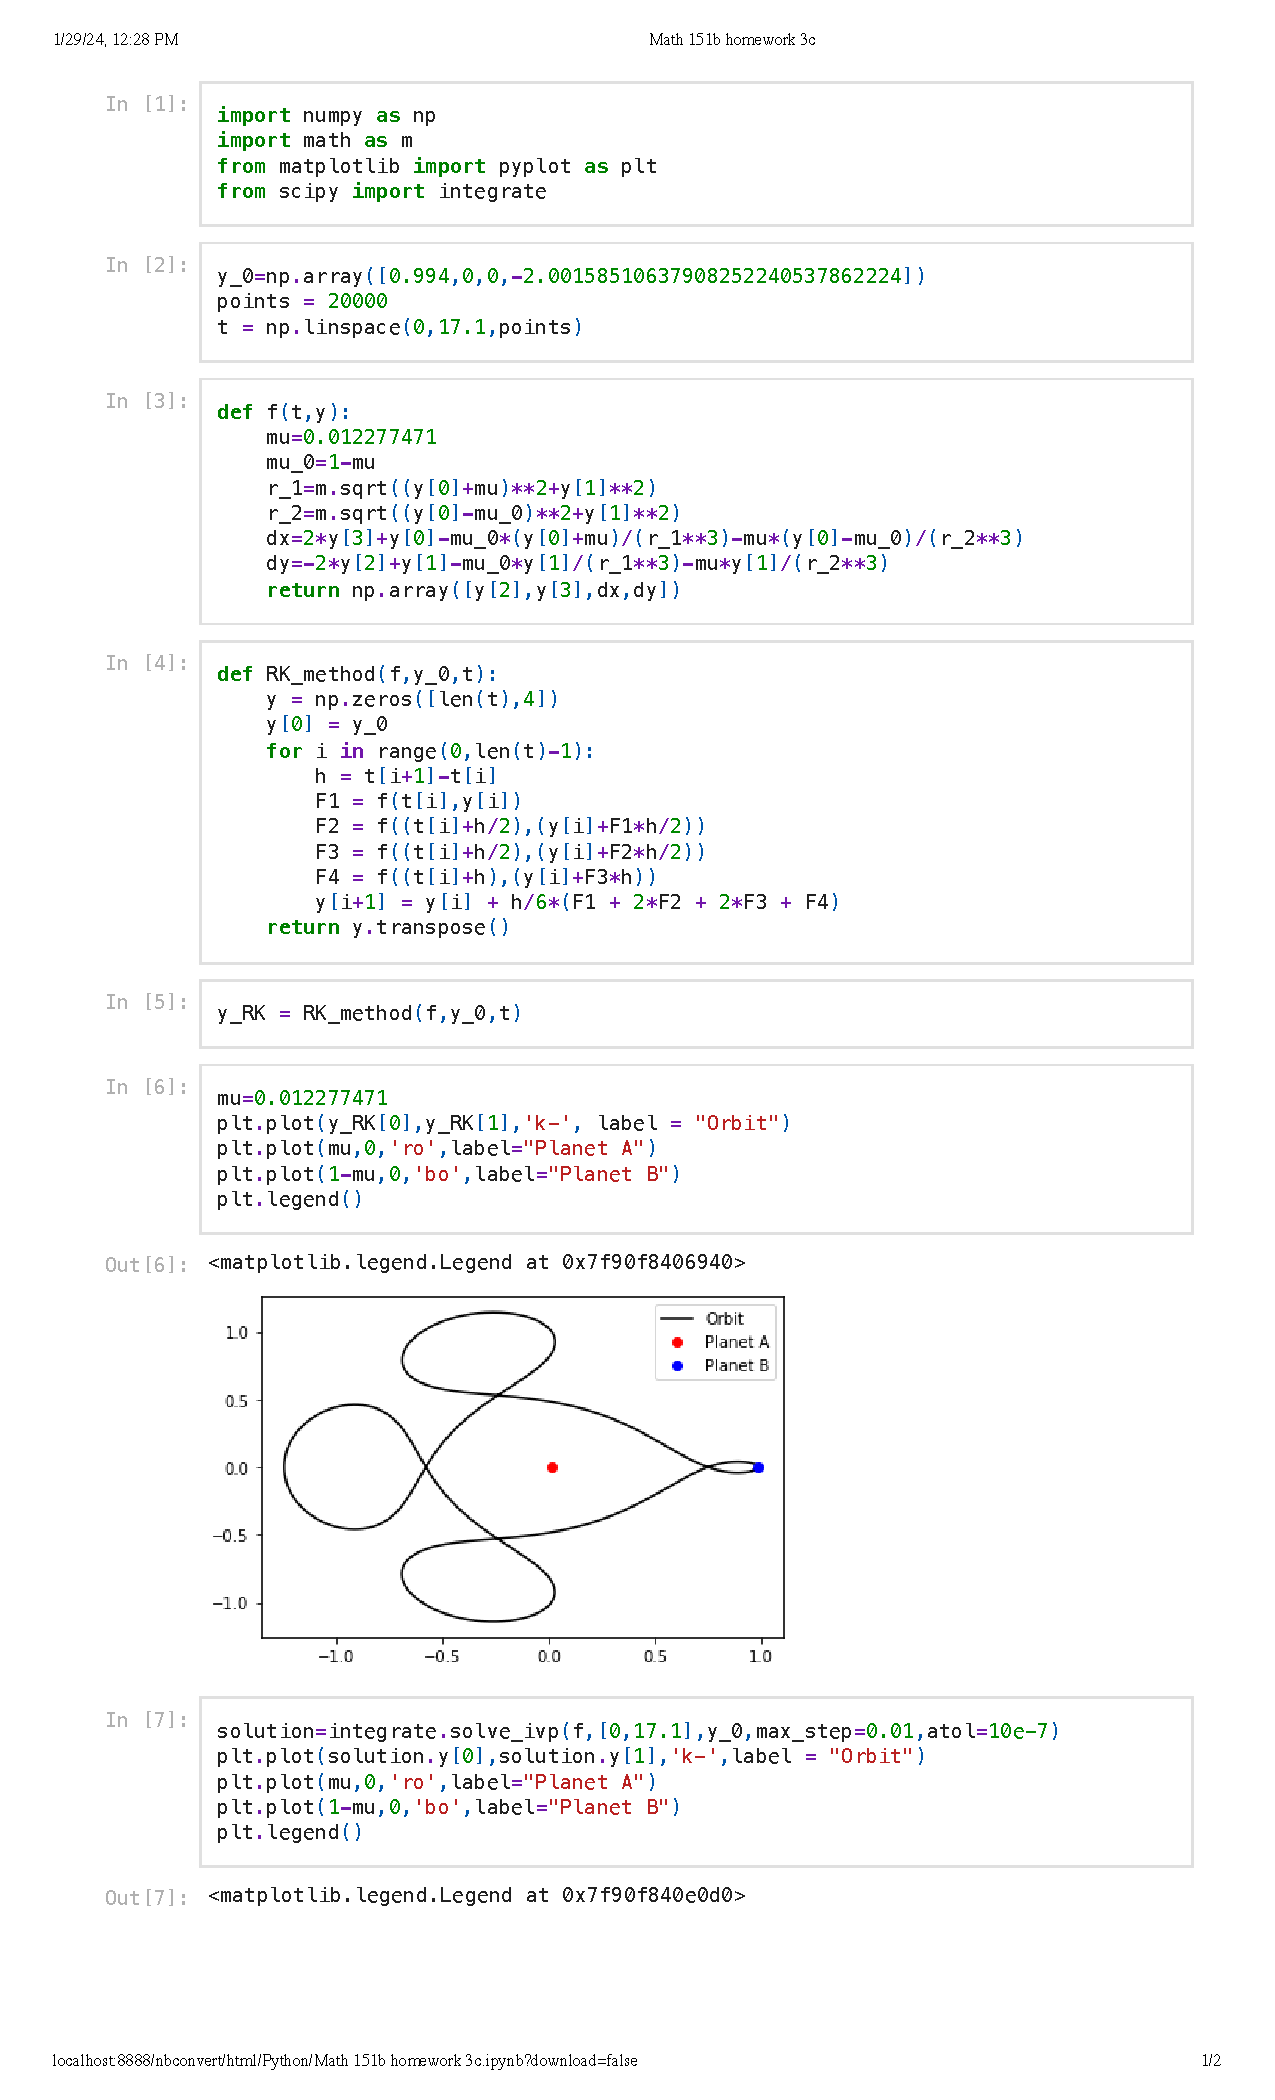
\includepdf[pages=-]{Math 151b homework 3c.pdf}
    \end{enumerate}
    
\end{enumerate}
\end{document}